% !TEX TS-program = XeLaTeX
% Commands for running this example:
% 	 xelatex slide
% 	bibtex8 -W -c cp1256fa slide
% 	xelatex slide
% 	xelatex slide
% End of Commands
% فایل پیکربندی اصلی اسلاید؛ که شامل بسته‌های استفاده شده و فونت‌های مربوط است.

\documentclass{beamer}

\usetheme{Boadilla} % Madrid Boadilla AnnArbor Warsaw Roechester % تم‌های بیمر با راست‌چین سازگار نیست!
%\usecolortheme{wolverine} % wolverine dove
\usefonttheme{serif} % این خط تغییری نکند

\usepackage{amssymb} % http://ctan.org/pkg/amssymb برای استفاده از سمبل‌ها و کاراکتر‌های خاص
\usepackage{pifont} % http://ctan.org/pkg/pifont برای استفاده از سمبل‌ها و کاراکتر‌های خاص
\usepackage{hyperref} % برای استفاده از ارجاعات

\usepackage{ragged2e} % برای استفاده از جاستیفای
\usepackage{color, colortbl} %  برای استفاده از رنگ‌های هایلایت شده در جداول
\usepackage{nameref} % برای نمایش نام ارجاع بجای شماره
\usepackage{tikz} % دیاگرام‌های تیکز
\usepackage[nonamebreak,square]{natbib} % nonamebreak,numbers,
\usepackage{smartdiagram} % برای ایجاد دیاگرام
\usepackage{graphicx} % 
\usepackage{booktabs} %
\usepackage{todonotes} % برای ایجاد یادداشت‌های مشابه با استیکی‌نوت
\usepackage{ptext} % 
\usepackage{xepersian} % 

\include{tashih} % تصحیحاتی که <<وفا خلیقی>> برای بیمر ایجاد کرد

\settextfont[Scale=0.9]{XB Niloofar} % B Bahij Nazanin, Lotus Lotus-Light
\setlatintextfont[Scale=.6]{XB Niloofar} % Linux Libertine O

\defpersianfont\nst[Scale=5.0]{IranNastaliq} %
\defpersianfont\bn[Scale=1.0]{Bahij Nazanin} %
\deflatinfont\tnr[Scale=1.0]{Times New Roman} %
\defpersianfont\shn[Scale=1.0]{Shekasteh_Beta} % شکسته نستعلیق
\defpersianfont\bsm[Scale=1.0]{S 110_Besmellah} %
\defpersianfont\msh[Scale=1.0]{B Mashhad} %
\deflatinfont\cnt[Scale=1.0]{Cantarell} % مناسب برای نوشتن کد برنامه‌سازی
\deflatinfont\lin[Scale=1.0]{Linux Libertine O} %
% ----------------------------------------------------------------------------

% دستورات اسلاید، مشابه با دستورات گزارش پایان‌نامه، در این بخش قرار می‌گیرد.

\definecolor{LRed}{rgb}{1,.8,.8}
\definecolor{MRed}{rgb}{1,.6,.6}
\definecolor{HRed}{rgb}{1,.2,.2}

\definecolor{Black}{rgb}{0,0,0} % equal to {0,0,0}
\definecolor{White}{rgb}{1,1,1} % equal to {255,255,255}
\definecolor{Red}{rgb}{1,0,0}
\definecolor{Lime}{rgb}{0,1,0}
\definecolor{Blue}{rgb}{0,0,1}
\definecolor{Yellow}{rgb}{1,1,0}
\definecolor{Cyan}{rgb}{0,1,1}
\definecolor{Magenta}{rgb}{1,0,1}
\definecolor{Silver}{rgb}{.75,.75,.75}
\definecolor{Gray}{rgb}{1,1,1}
\definecolor{Maroon}{rgb}{1,0,0}
\definecolor{Olive}{rgb}{1,1,0}
\definecolor{Green}{rgb}{0,1,0}
\definecolor{Purple}{rgb}{1,0,1}
\definecolor{Teal}{rgb}{0,1,1}
\definecolor{Navy}{rgb}{0,0,1}
\definecolor{Orange}{rgb}{1,.65,0}
% --------------------------------------------------------------------------
% http://ctan.org/pkg/amssymb
% http://ctan.org/pkg/pifont
\newcommand{\cmark}{\ding{51}}% تیک؛ کد سمبل از پی‌دی‌اِف مرجع استخراج شده
\newcommand{\xmark}{\ding{55}}% زبدر
% ----------------------------------------------------------------------------
\title[
عنوان ۳-۴ کلمه‌ای]{عنوان کامل و طولانی فقط برای نمایش در صفحه اول}
\author{نام دانشجو}
\institute[نام دانشگاه]
{
نام دانشگاه\\
\medskip
\lin\textit{some-one@provider.domain}
}
\date{تاریخ روز دفاع} 
% ----------------------------------------------------------------------------

\begin{document}
\label{front_cover}

\section{شروع}
\subsection{عنوان}
\begin{frame}
\maketitle
\end{frame}

% بد نیست که جلسه دفاع، با یک نقل قول مناسب، از یکی از بزرگان شروع شود. این به جلسه شما، حال‌و‌هوای علمی‌ می‌دهد. چون گزارش من، حدودا در شاخه مهندسی نرم‌افزار قرار می‌گرفت از یکی از سخنان آقای <<کیپرز جونز>> استفاده کردم. میشه از سایت‌هایی مثل: https://www.inspiringquotes.us ، http://www.azquotes.com/ یا https://www.brainyquote.com/ نیز استفاده کرد.

\label{quote}
\subsection{در آغاز}

\begin{frame}
\frametitle{در آغاز}

\pause
\begin{columns}[c]
\column{.45\textwidth} % Left column and image
\justify \lr{\lin\fontsize{11}{13.2}\selectfont{"High-quality software is not expensive. High-quality software is faster and cheaper to build and maintain than low-quality software, from initial development all the way through total cost of ownership."}}
\flushright{\lr{\citep{Jones:2011:ESQ:2025240}}} 

\column{.52\textwidth} % Right column and quote
\begin{figure}
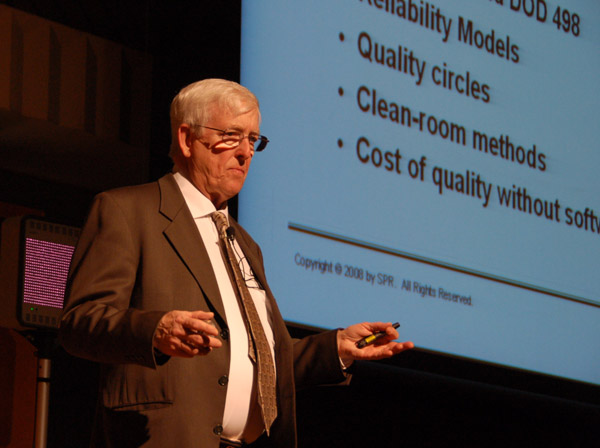
\includegraphics[scale=.3]{resources/img/capers-jones-001.jpg}
\end{figure}
\bigskip
\end{columns}

\end{frame}

\section{کلیات}
\label{understanding_problem}

\subsection{تعریف مساله}
\begin{frame}
\frametitle{تعریف مساله}

\begin{itemize}\raggedleft
\begin{RTLitems}
\item
عبارت ۱.
\pause
\item
عبارت ۲.
\pause
\item
عبارت ۳.
\pause

\flushright{جمله نتیجه‌گیری}
\pause
\end{RTLitems}
\end{itemize}

\end{frame}

\label{main_questions_and_study_hypothesis}

\subsection{سوال‌های اصلی و فرضیات}
\begin{frame}
\frametitle{سوال‌ها و فرضیه‌های تحقیق}

\begin{enumerate}\raggedleft
\begin{RTLitems}
\item سوال اول؟
\pause
\item سوال دوم؟
\pause
\item سوال سوم؟
\pause
\end{RTLitems}
\end{enumerate}

%\todo{فرضیه‌ها را چگونه در سوالات برجسته کنیم ؟؟}

\end{frame}

\label{study_necessity}

\subsection{سابقه تحقیق}
\begin{frame}
\frametitle{سابقه تحقیق}
\pause
ترجیحا با یک دیاگرام (\lr{smartdiagram}) این گذر زمانی، نمایش داده شود.
\end{frame}

%\lr{\cite{}}


%\label{study_necessity}

\subsection{روش تحقیق}
\begin{frame}
\frametitle{روش تحقیق}



\end{frame}
 % روش تحقیق، برای جلوگیری از سوالات اضافی(!) حذف شد
\label{study-how_its_done}

\subsection{مراحل انجام کار}
\begin{frame}
\frametitle{مراحل انجام کار}

\pause
\raggedleft{تعداد مراحل:}

\begin{enumerate}\raggedleft
\begin{RTLitems}
\item 
مرحله ۱
\pause
\item 
مرحله ۲
\pause
\end{RTLitems}
\end{enumerate}

\end{frame}

\label{study_applications}

\subsection{کاربردها}
\begin{frame}
\frametitle{کاربردها}

\begin{itemize}\raggedleft
\begin{RTLitems}
\item
کاربرد ۱
\pause
\item 
کاربرد ۲
\pause
\item 
کاربرد ۳
\pause
\end{RTLitems}
\end{itemize}

\end{frame}

%\section{پیشینه} % 
% نیازی به نوشتن پیشینه نیست! اصولا بدون این پیشینه‌ هم، زمان دفاع کافی نیست. 
\section{مرور ادبیات}
\label{architectural_problems_literature}

\subsection{مرور ادبیات کاستی‌های معماری}
\begin{frame}
\frametitle{مرور ادبیات کاستی‌های معماری}

\raggedleft{سوال ورود به ادبیات؟}
\pause
\begin{enumerate}\raggedleft
\begin{RTLitems}
\item
عبارت اولی
\pause
\item
عبارت دومی
\pause
\end{RTLitems}
\end{enumerate}

\end{frame}

\section{معرفی موضوع پیشنهادی}
\label{introduction_to_suggested_detection_platform}

\subsection{معرفی چیز پیشنهادی}
\begin{frame}
\frametitle{معرفی چیز پیشنهادی}

\pause

من اینجا دوتا عکس نمایش دادم و روی عکس‌ها، شروع به توضیح کردم. دوست داشتین، شمام می‌تونین. :-)

%\begin{center}
%\begin{tikzpicture}[remember picture,overlay]
%  \node[xshift=+0cm,yshift=-.25cm] (img1) {\includegraphics[scale=0.28]{resources/img/... .png}};
%  \pause
%  \node[xshift=+0cm,yshift=-.5cm] (img2) {\includegraphics[scale=1.03]{resources/img/... .jpg}};
%\end{tikzpicture}
%\end{center}

\end{frame}

\section{ارزیابی}
\label{answering_main_questions_and_study_hypothesis}

\subsection{پاسخ به سوالات اصلی و راستی‌آزمایی فرضیه‌ها}
\begin{frame}
\frametitle{پاسخ به سوالات اصلی و راستی‌آزمایی فرضیه‌ها}

\pause
\begin{block}{۱. متن سوال اول؟}

\pause
پاسخ به اولین سوال؛ راستش من در آیتمایز جواب دادم.
\end{block}

\pause
\begin{block}{۲. متن سوال دوم؟}
\pause

پاسخ به سوال دوم ...
\end{block}

\pause
\begin{block}{۳. متن سوال سوم؟}
\pause

اینم آخرین پاسخ.
\end{block}

\end{frame}

\section{پیشنهادها}
\label{conclusions_and_future_works}

\subsection{پیشنهادات آتی}
\begin{frame} 
\frametitle{پیشنهادات آتی}

\pause
یه سری حرفای خوووووووب!
\end{frame}

\label{final_words}

\section{قدردانی}
\subsection{سخن آخر}
\begin{frame}
\frametitle{سخن آخر}

\pause
\begin{center}
{\nst \fontsize{6}{7.2}\selectfont {
با سپاس از سروران گرامی؛
}}
\end{center}

\end{frame}

\section{ذخیره}
\label{bibliography}

\subsection{منابع}
\begin{frame}%[t,allowframebreaks]
\frametitle{منابع}

\bibliographystyle{asa-fa} % plain-fa-inLTR-beamer
\bibliography{references}‬ ‫

\end{frame}
 % در صورت وجود ارجاعات به منابع، لیست منابع در انتها آورده شود.
% برای انجام دفاع بهتر، اسلایدهای رزرو (پاسخ مناسب به سوالات پیش‌بینی شده) در این بخش ایجاد شود.
\end{document}

